% !TEX root = ../main.tex
\section*{Backup Slides}
\begin{frame}{}
    \centering \Huge{\ef{Backup Slides}}
\end{frame}

% TODO. Re-order these up once the main presentation is finished.
\subsection*{CCDB}
% !TEX root = ../main.tex
% --+ 20.01 CCDB +--------------------------------------------------------------
\begin{frame}{Calibration Constants Database}
    \label{20.01::ccdb}
    \begin{itemize}
        \item
        \vspace{12pt}
        In simple terms, the Calibration Constants Database (CCDB) is a central repository where the CLAS12 \ef{calibration constants} are stored.
        \item
            The stored data includes geometry constants, corrections for different imperfections, drifts in the electronics, etc.

        \vspace{12pt}
        \item
            A CCDB \ef{variation} (e.g. \eft{rgf\_spring2020}) is a ``version'' of the CCDB for a particular experiment season.

        \vspace{12pt}
        \item
            In addition, there are special variations for gemc simulations (e.g. \eft{rgf\_spring2020\_mc}), so as to not include calibration data from the real world into the simulation world.
    \end{itemize}

    \backref{11.42::alignment_effect}
\end{frame}


\subsection*{FMT Acceptance Curve}
% !TEX root = ../main.tex
% --+ 20.02 FMT ACCEPTANCE CURVE +----------------------------------------------
\begin{frame}{FMT Acceptance Curve}
    \label{20.02::fmt_acceptance_curve}
    \begin{center}
        \animategraphics[loop,controls,width=0.8\linewidth]{10}{theta_z/frame-}{0}{132}
    \end{center}

    \backref{11.43::geometry_effect_1}
\end{frame}


\subsection*{FMT Efficiency Error Estimation}
% !TEX root = ../main.tex
% --+ 20.03 FMT EFFICIENCY ERROR ESTIMATION +-----------------------------------
\begin{frame}{FMT Efficiency Error Estimation}
    \label{20.03::fmt_efficiency_error_estimation}

    \vspace{18pt}

    We define \ef{$P(L_n)$} as the probability of layer \ef{$n$} detecting a particle.
    Assuming all layers have the same efficiency \ef{$E_1$},
    \begin{equation*}
        P(L_1) = P(L_2) = P(L_3) = E_1,
    \end{equation*}
    the efficiency for 3-layer tracks \ef{$E_3$} can be obtained using \ef{$P(L_n)$} as follows
    \begin{align}
        E_3 &= P(L_1)P(L_2)P(L_3)
        \nonumber \\
        E_3 &= E_{1(3)}^3,
        \label{eq::14.14::efficiency3}
    \end{align}
    where \ef{$E_{1(3)}$} is the 1-layer efficiency estimated from 3-layer tracks.

    \vspace{18pt}

    From \eqref{eq::14.14::efficiency3}, we can estimate \ef{$E_{1(3)}$} as
    \begin{equation}
        E_{1(3)} = \sqrt[3]{E_3}.
        \label{eq::14.14::efficiency1(3)}
    \end{equation}

    \backref{11.45::reconstruction_effect}
\end{frame}

\begin{frame}{FMT Efficiency Error Estimation}
    \vspace{18pt}

    For 2-layer tracks, the efficiency \ef{$E_2$} can be obtained as
    \begin{align}
        E_2 &= P(L_1)P(L_2)\left(1 - P(L_3)\right)                \nonumber \\
             &\hspace{24pt} + P(L_2)P(L_3)\left(1 - P(L_1)\right) \nonumber \\
             &\hspace{24pt} + P(L_3)P(L_1)\left(1 - P(L_2)\right) \nonumber \\
             &\hspace{24pt} + P(L_1)P(L_2)P(L_3)                  \nonumber \\
        E_2 &= 3E_{1(2)}^2\left(1 - E_{1(2)}\right) + E_{1(3)}^3
            \nonumber \\
        E_2 &= 3E_{1(2)}^2 \cdot \left( 1 - E_{1(2)} \right) + E_3,
        \label{eq::14.14::efficiency2}
    \end{align}
    where \ef{$E_{1(2)}$} is the 1-layer efficiency estimated from 2-layer tracks.

    \vspace{18pt}

    \ef{$E_{1(2)}$} cannot be obtained explicitly from \eqref{eq::14.14::efficiency2}, but we can estimate it numerically.

    \backref{11.45::reconstruction_effect}
\end{frame}

\begin{frame}{FMT Efficiency Error Estimation}
    \vspace{18pt}

    Using Equations \eqref{eq::14.14::efficiency2} and \eqref{eq::14.14::efficiency1(3)}, we can estimate the weighted average efficiency \ef{$\xoverline{E_1}$} as
    \begin{equation*}
        \xoverline{E_1} = \frac{4E_{1(2)} + E_{1(3)}}{5},
    \end{equation*}
    where the weights are assigned based on the number of ways 2 and 3-layer tracks can be obtained, 4 and 1, respectively.

    \vspace{18pt}

    From \ef{$\xoverline{E_1}$}, we can estimate the errors on \ef{$E_{1(2)}$} and \ef{$E_{1(3)}$} as
    \begin{align*}
        \delta(E_{1(2)}) = |\xoverline{E_1} - E_{1(2)}|, \\
        \delta(E_{1(3)}) = |\xoverline{E_1} - E_{1(3)}|.
    \end{align*}

    \backref{11.45::reconstruction_effect}
\end{frame}

\begin{frame}{FMT Efficiency Error Estimation}
    To propagate these errors to the efficiencies \ef{$E_2$} and \ef{$E_3$}, we use the variance formula
    \begin{equation*}
        \delta\left(f(x)\right) = \frac{\partial f(x)}{\partial x} \cdot \delta(x),
    \end{equation*}
    where \ef{$\delta(E_2)$}, obtained from Equation \eqref{eq::14.14::efficiency2}, is
    \begin{align*}
        \delta(E_2) &= \frac{\partial}{\partial E_{1(2)}} \left( 3E_{1(2)}^2 - 3E_{1(2)}^3 + E_{1(3)}^3 \right)
            \cdot \delta \left( E_{1(2)} \right) \\
        \delta(E_2) &= \left( 6E_{1(2)} - 9E_{1(2)}^2 \right) \cdot \delta \left( E_{1(2)} \right)
    \end{align*}
    and \ef{$\delta(E_3)$}, obtained from Equation \eqref{eq::14.14::efficiency3}, is
    \begin{align*}
        \delta(E_3) &= \frac{\partial}{\partial E_{1(3)}} \left( E_{1(3)}^3 \right) \cdot \delta \left( E_{1(3)} \right) \\
        \delta(E_3) &= 3E_{1(3)}^2 \cdot \delta \left( E_{1(3)} \right).
    \end{align*}

    \backref{11.45::reconstruction_effect}
\end{frame}


\subsection*{FMT Efficiency Study}
% !TEX root = ../main.tex
% --+ 20.04 FMT EFFICIENCY STUDY +----------------------------------------------
\begin{frame}{FMT Efficiency Study}
    \label{20.04::fmt_efficiency_study}
    \begin{itemize}
        \item
            Then, to see how these efficiency effects affects the different DIS variables, we need to understand their behavior in

            \vspace{6pt}
            \begin{itemize}
                \item
                    vertex z position (\ef{$v_z$}),

                \item
                    polar angle (\ef{$\theta$}),

                \item
                    azimuthal angle (\ef{$\varphi$}), and

                \item
                    momentum (\ef{$p$}).
            \end{itemize}

        \vspace{12pt}
        \item
            Based on the geometry cut, we expect a strong dependence on \ef{$v_z$} and \ef{$\theta$}, and at most a weak one on \ef{$\varphi$} and \ef{$p$}.
    \end{itemize}

    \vspace{12pt}
    \ef{*}All plots presented in this appendix are from \ef{run 12016}.

    \backref{11.44::reconstruction_effect}
\end{frame}

\begin{frame}{FMT Efficiency Study: $v_z$}
    \begin{center}
        \vspace{-6pt}
        \begin{figure}[t]
            \centering{
                \fbox{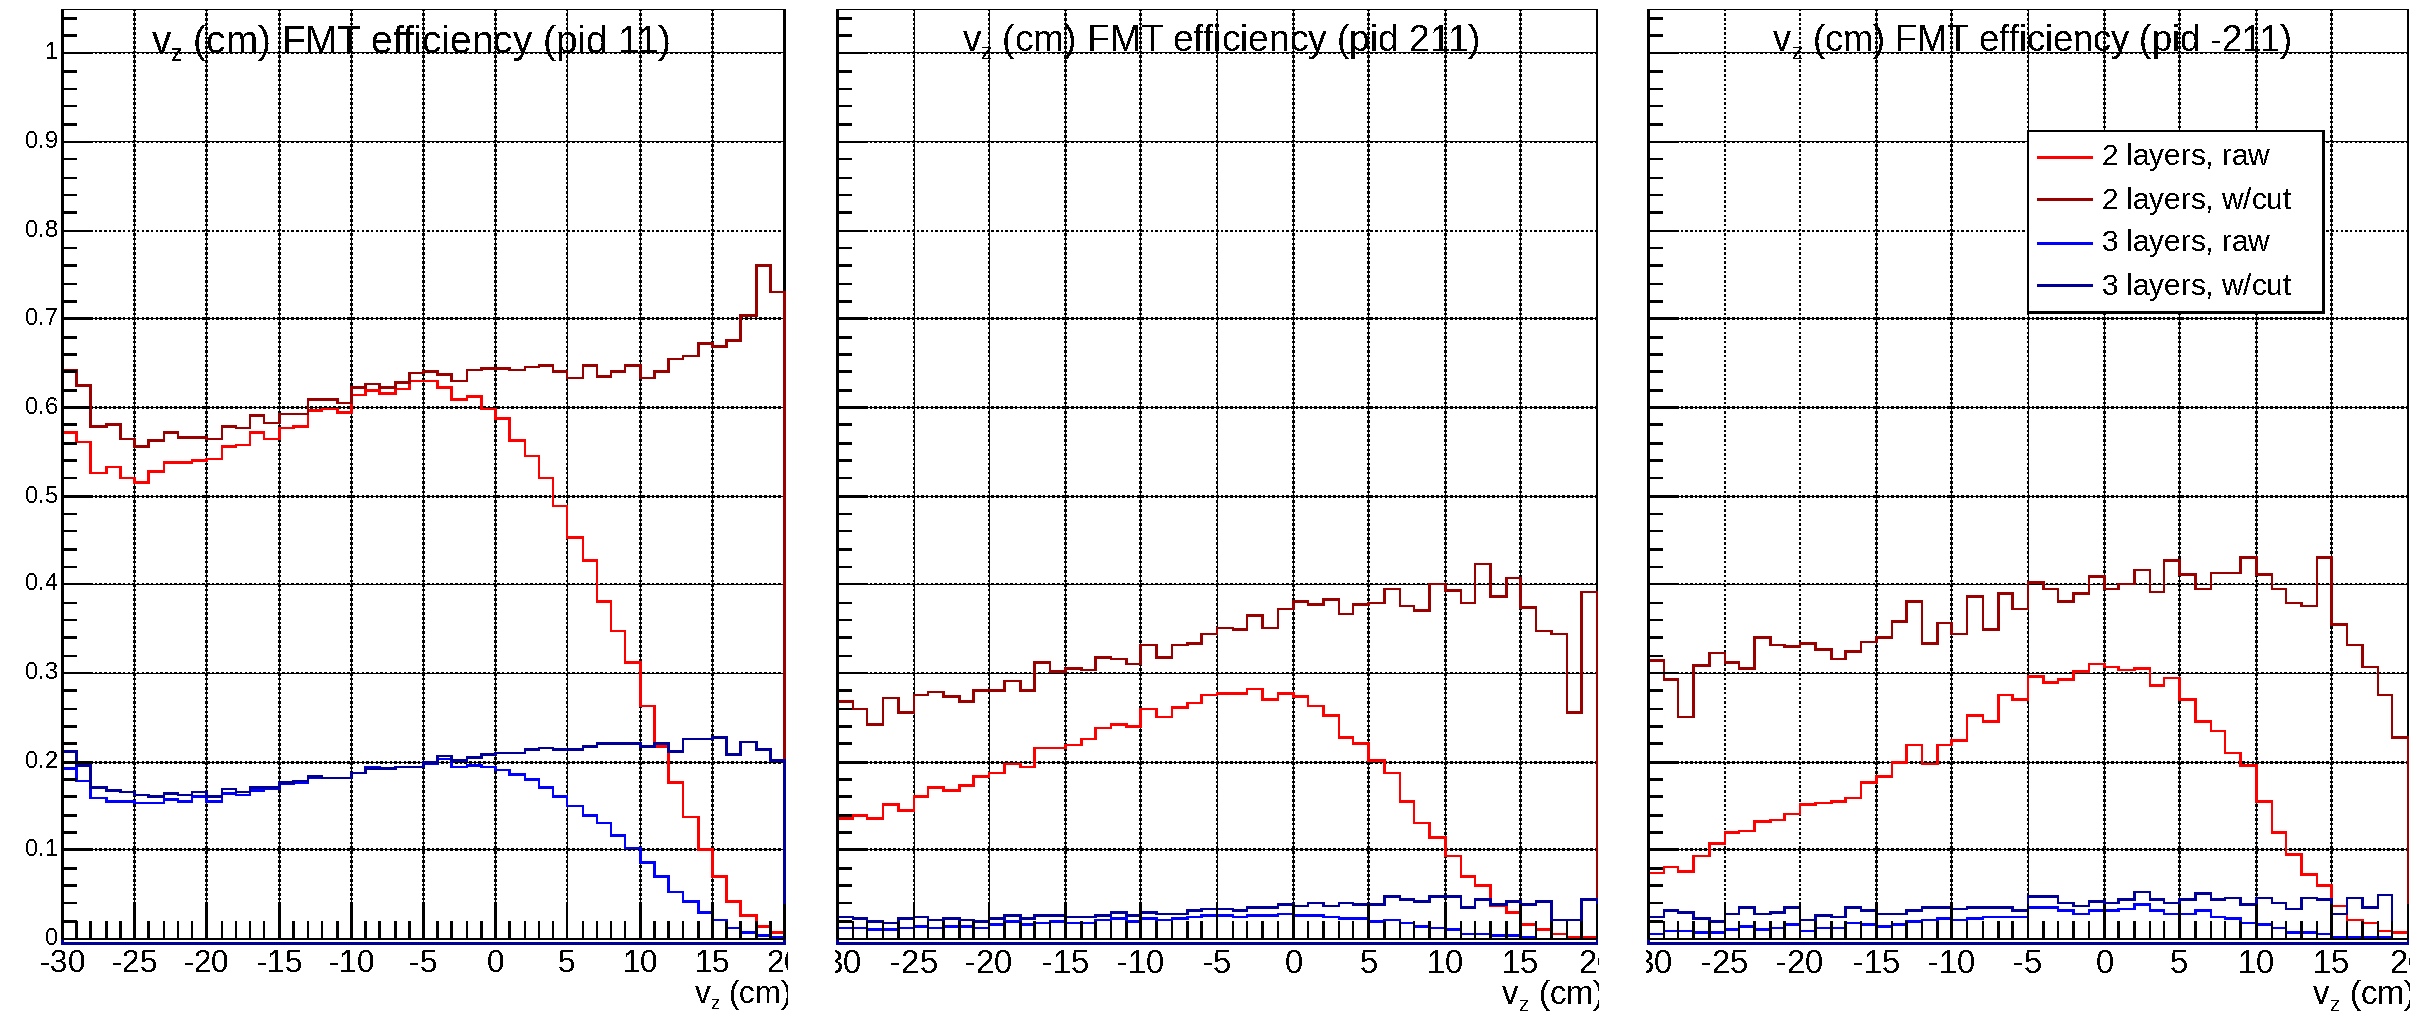
\includegraphics[width=0.98\textwidth]{04eff_vz.pdf}}
            }
        \end{figure}
        \scriptsize{\textit{Efficiency over \ef{$v_z$} for $e^-$, $\pi^+$, and $\pi^-$.}}
    \end{center}

    \backref{11.44::reconstruction_effect}
\end{frame}

\begin{frame}{FMT Efficiency Study: $\theta$}
    \begin{center}
        \vspace{-6pt}
        \begin{figure}[t]
            \centering{
                \fbox{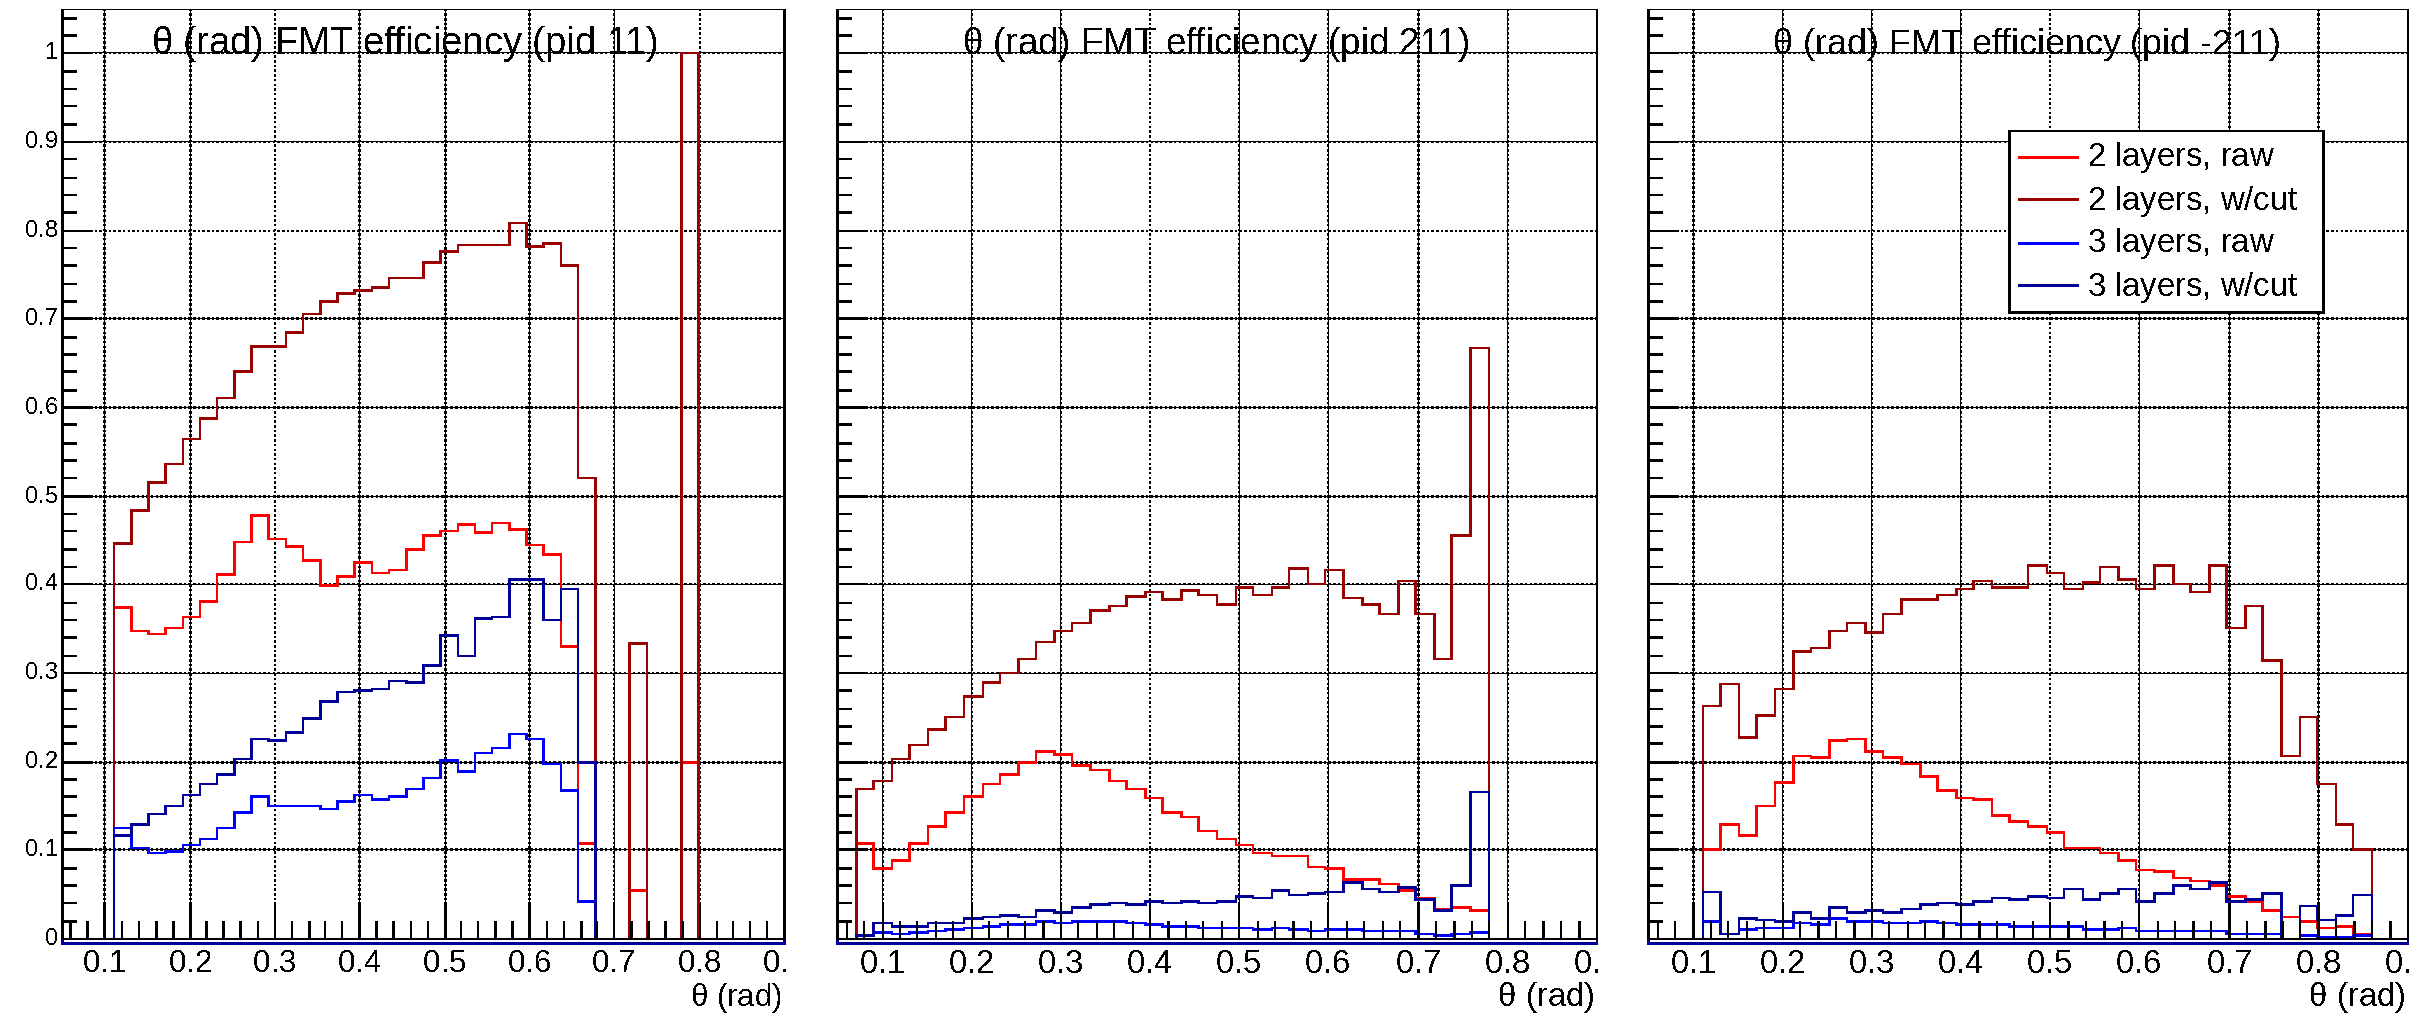
\includegraphics[width=0.98\textwidth]{04eff_theta.pdf}}
            }
        \end{figure}
        \scriptsize{\textit{Efficiency over \ef{$\theta$} for $e^-$, $\pi^+$, and $\pi^-$.}}
    \end{center}

    \backref{11.44::reconstruction_effect}
\end{frame}

\begin{frame}{FMT Efficiency Study: $p$}
    \begin{center}
        \vspace{-6pt}
        \begin{figure}[t]
            \centering{
                \fbox{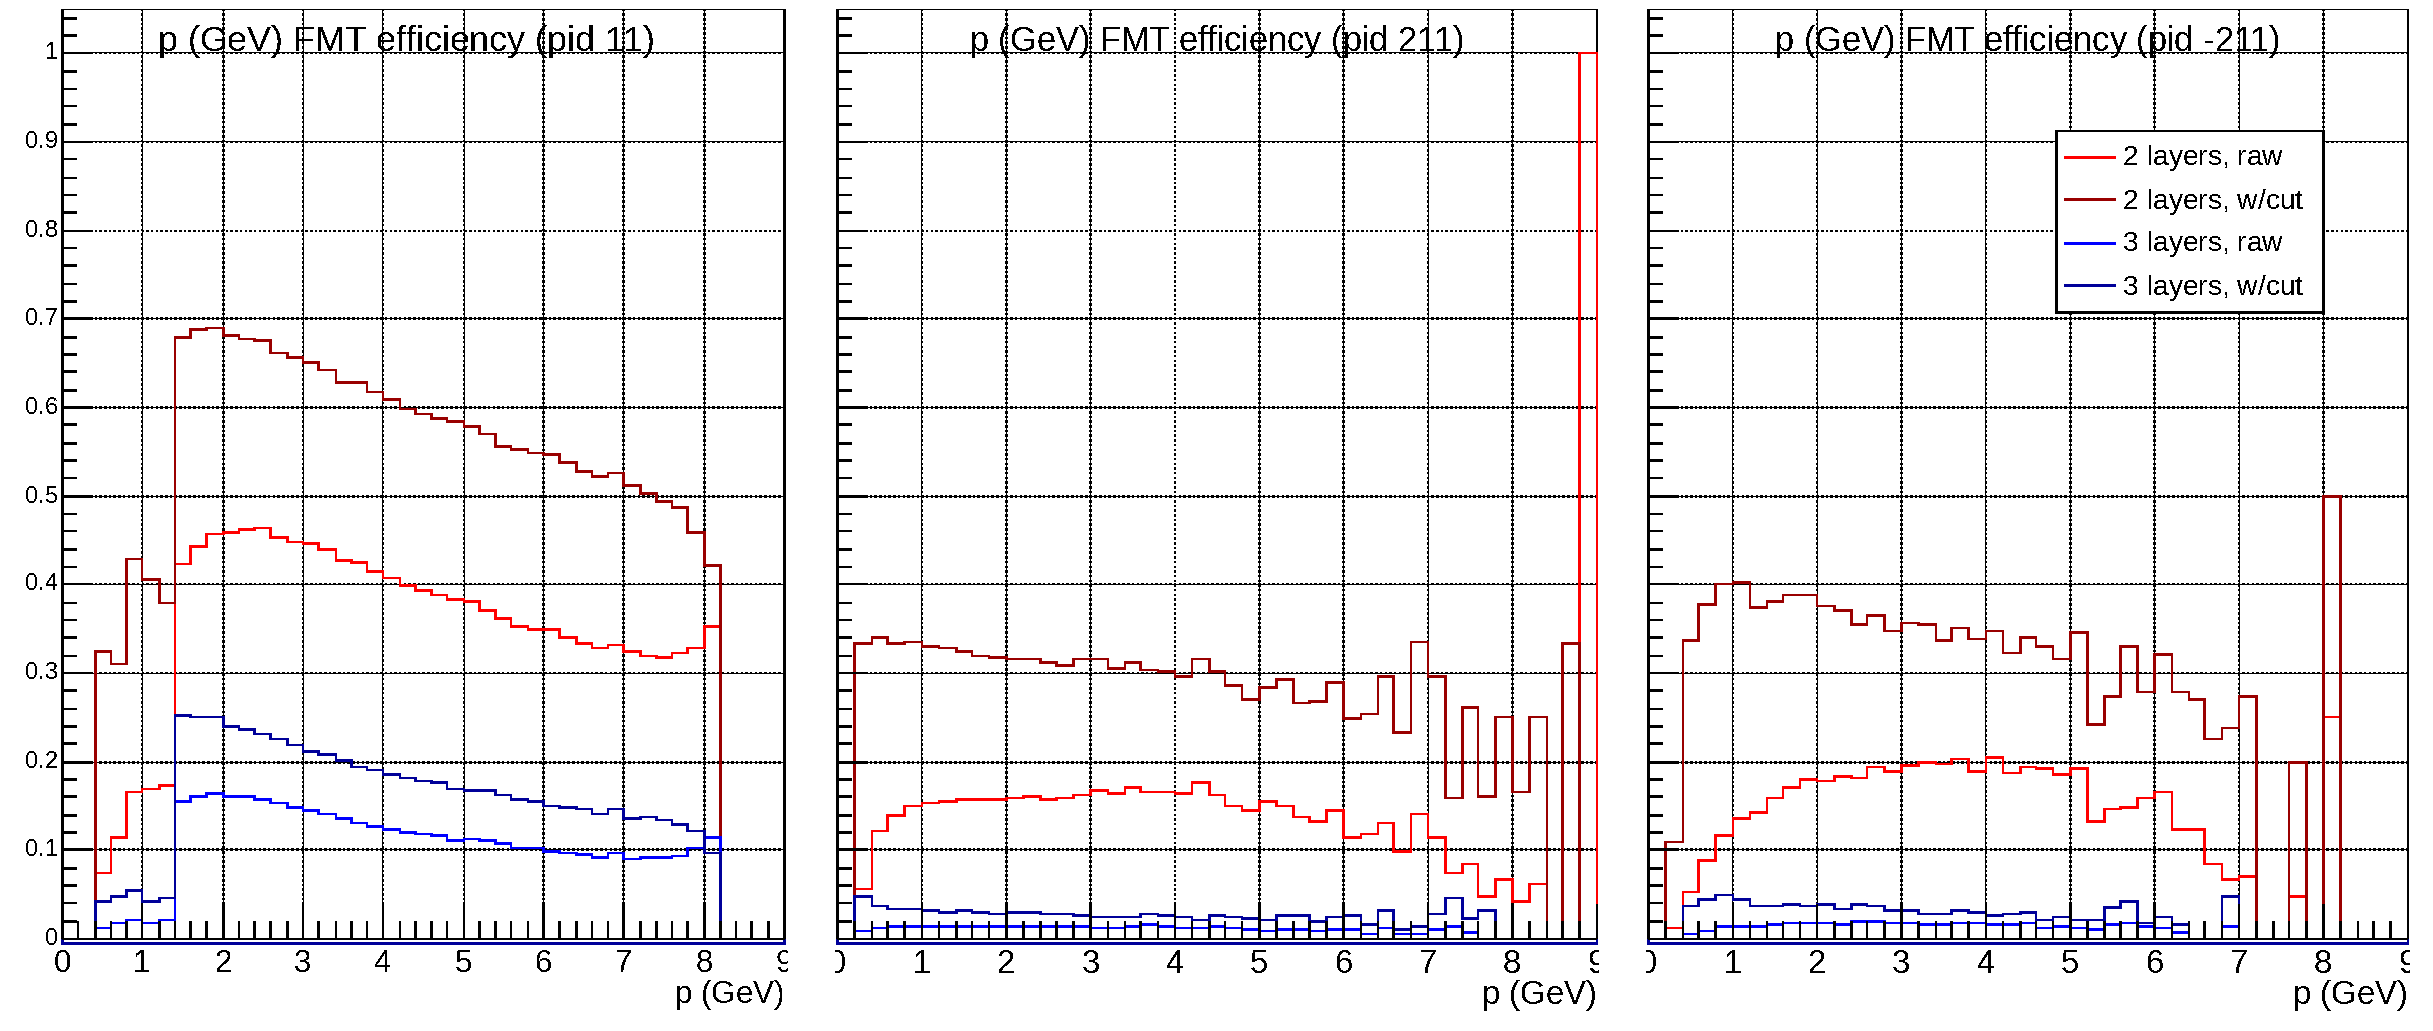
\includegraphics[width=0.98\textwidth]{04eff_p.pdf}}
            }
        \end{figure}
        \scriptsize{\textit{Efficiency over \ef{$p$} for $e^-$, $\pi^+$, and $\pi^-$.}}
    \end{center}

    \backref{11.44::reconstruction_effect}
\end{frame}

\begin{frame}{FMT Efficiency Study: $\varphi$}
    \begin{center}
        \vspace{-6pt}
        \begin{figure}[t]
            \centering{
                \fbox{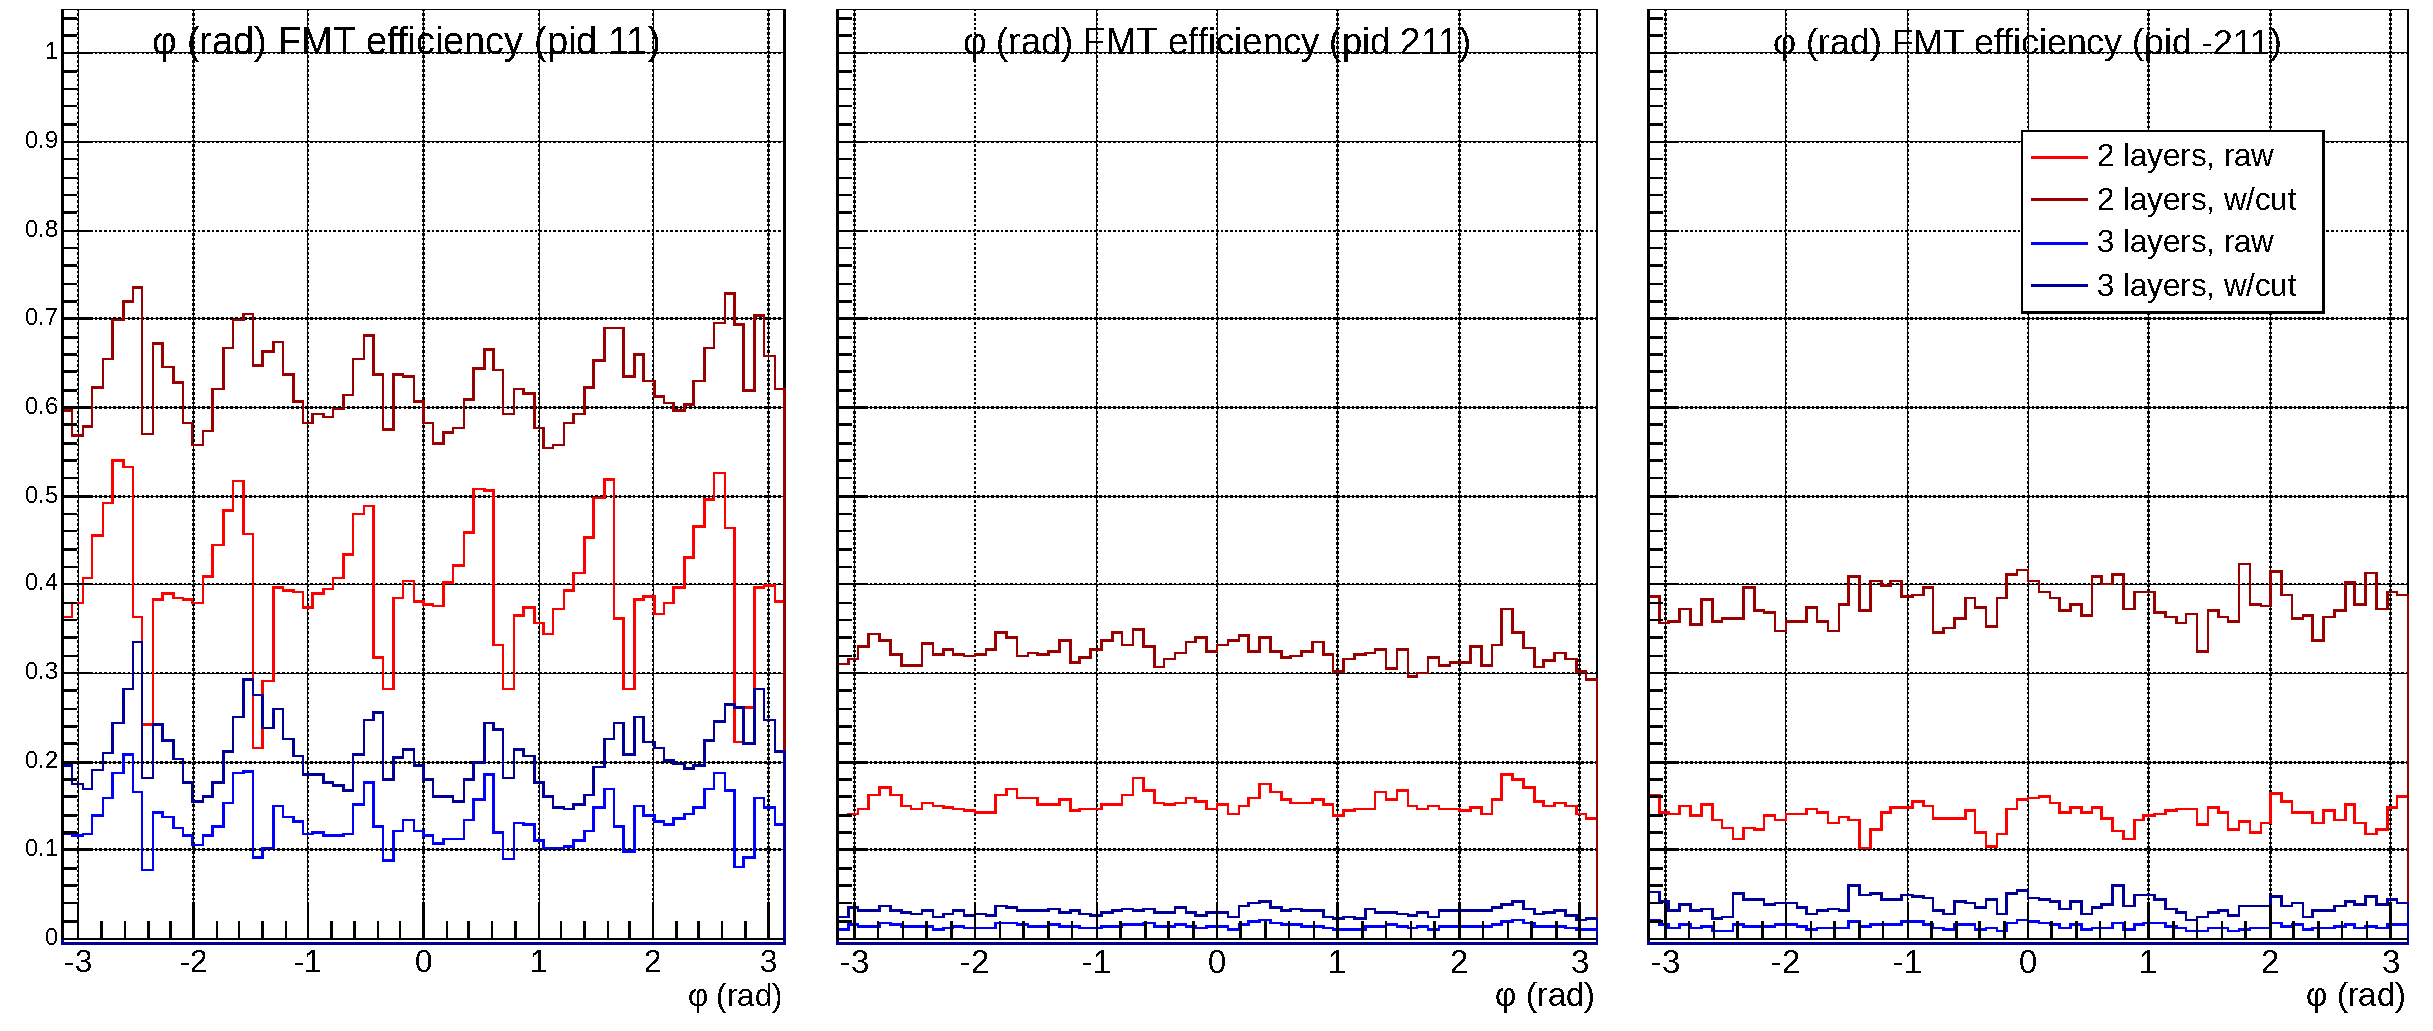
\includegraphics[width=0.98\textwidth]{04eff_phi.pdf}}
            }
        \end{figure}
        \scriptsize{\textit{Efficiency over \ef{$\varphi$} for $e^-$, $\pi^+$, and $\pi^-$.}}
    \end{center}

    \backref{11.44::reconstruction_effect}
\end{frame}

\begin{frame}{FMT Efficiency Study: $\varphi$}
    \label{20.04::fmt_efficiency_study_end}

    The loss of the sharp dips in $e^-$ \ef{$\varphi$} efficiency can be explained by the loss of DC tracks upon applying the cut.

    \begin{center}
        \begin{figure}[t]
            \centering{
                \fbox{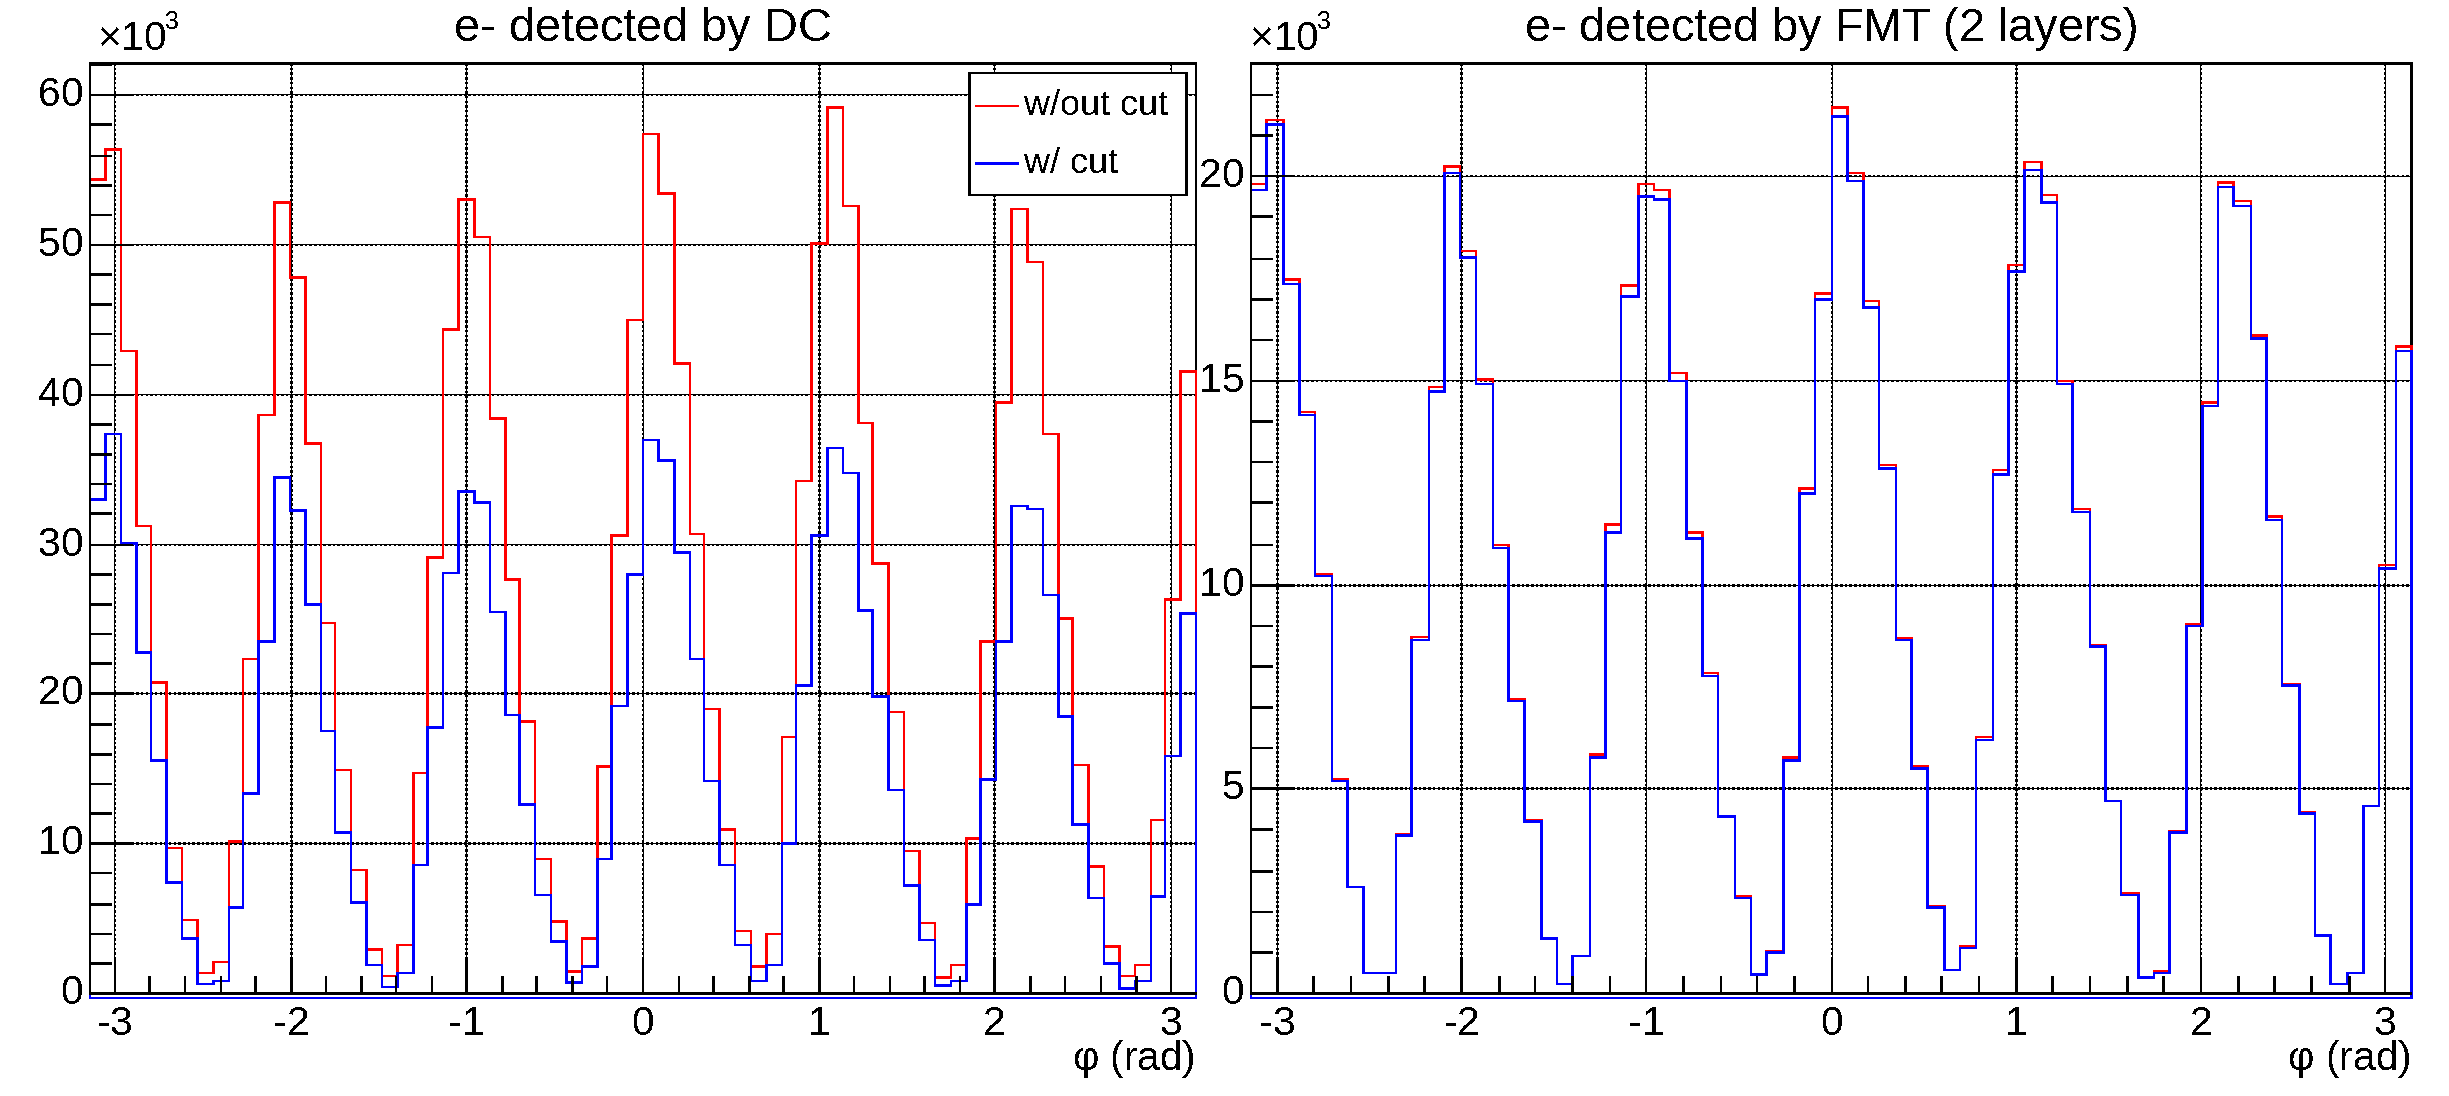
\includegraphics[width=0.98\textwidth]{04gcut_phi.pdf}}
            }
        \end{figure}
    \end{center}

    \backref{11.44::reconstruction_effect}
\end{frame}


\subsection*{Acceptance Error Estimation}
% !TEX root = ../main.tex
% --+ 20.05 ACCEPTANCE ERROR ESTIMATION +---------------------------------------
\begin{frame}{Acceptance Error Estimation}
    \label{20.05::acceptance_error_estimation}

    The acceptance fraction is computed as follows
    \begin{equation}
        y_\text{acc} = \frac{y_r}{y_t},
        \label{eq::14.20::acc}
    \end{equation}
    where \ef{$y_\text{acc}$} is the percentage of accepted particles, \ef{$y_r$} is the number of reconstructed particles, and \ef{$y_t$} is the number of thrown particles.

    \vspace{6pt}

    Then, to propagate the error of \ef{$y_r$} (\ef{$e_d$}) and \ef{$y_t$} (\ef{$e_t$}) to \ef{$y_\text{acc}$} (\ef{$e_\text{acc}$}), we have
    \begin{align}
        e_\text{acc} &= \delta \left(\frac{y_r}{y_t}\right)
        \nonumber \\
        &= y_\text{acc} \cdot \sqrt{
            \left( \frac{e_r}{y_r} \right)^2 + \left( \frac{e_t}{y_t} \right)^2
        },
        \nonumber
        \intertext{since \ef{$y_t$} is the number of trials, we can assume \ef{$e_t = 0$}, and thus}
        &= y_\text{acc} \cdot \frac{e_r}{y_r}.
        \label{eq::14.20::acc_error_estimation}
    \end{align}

    \backref{11.52::electron_variables}
\end{frame}

\begin{frame}{Acceptance Error Estimation}
    \label{20.05::acceptance_error_estimation_end}

    From the Central Limit Theorem, assuming a normal distribution, the variance \ef{$e_r^2$} is given by
    \begin{equation*}
        e_r^2 = y_t \cdot y_\text{acc} (1 - y_\text{acc}).
    \end{equation*}

    \vspace{12pt}

    Replacing this in Equation \eqref{eq::14.20::acc_error_estimation}, we obtain
    \begin{equation*}
        e_\text{acc} = y_\text{acc} \cdot \frac{\sqrt{y_t y_\text{acc}(1 - y_\text{acc})}}{y_r}.
    \end{equation*}

    \vspace{12pt}

    Now, replacing \ef{$y_\text{acc}$} with its definition from Equation \eqref{eq::14.20::acc}, we arrive at the final error expression
    \begin{equation}
        e_\text{acc} = \sqrt{\frac{y_\text{acc}(1-y_\text{acc})}{y_t}}.
        \label{eq::14.20::acc_error}
    \end{equation}

    \backref{11.52::electron_variables}
\end{frame}


\subsection*{Fiducial Cuts}
% !TEX root = ../main.tex
\begin{frame}{Fiducial Cuts}
    \label{20.06::fiducial_cuts}

    \vspace{48pt}

    \begin{itemize}
        \item
            To apply fiducial cuts, we would provide \ef{$\phi$} vs. \ef{$\theta$} curves that cut events at the edges of each DC sector.

        \vspace{18pt}
        \item
            One curve would be needed for each \ef{$p$} bin, for each sector.

        \vspace{18pt}
        \item
            This would be done for each PID processed.
    \end{itemize}

    \backref{11.21::summary}
\end{frame}

\begin{frame}{Fiducial Cuts}
    \begin{center}
        \begin{figure}[t]
            \centering{
                \fbox{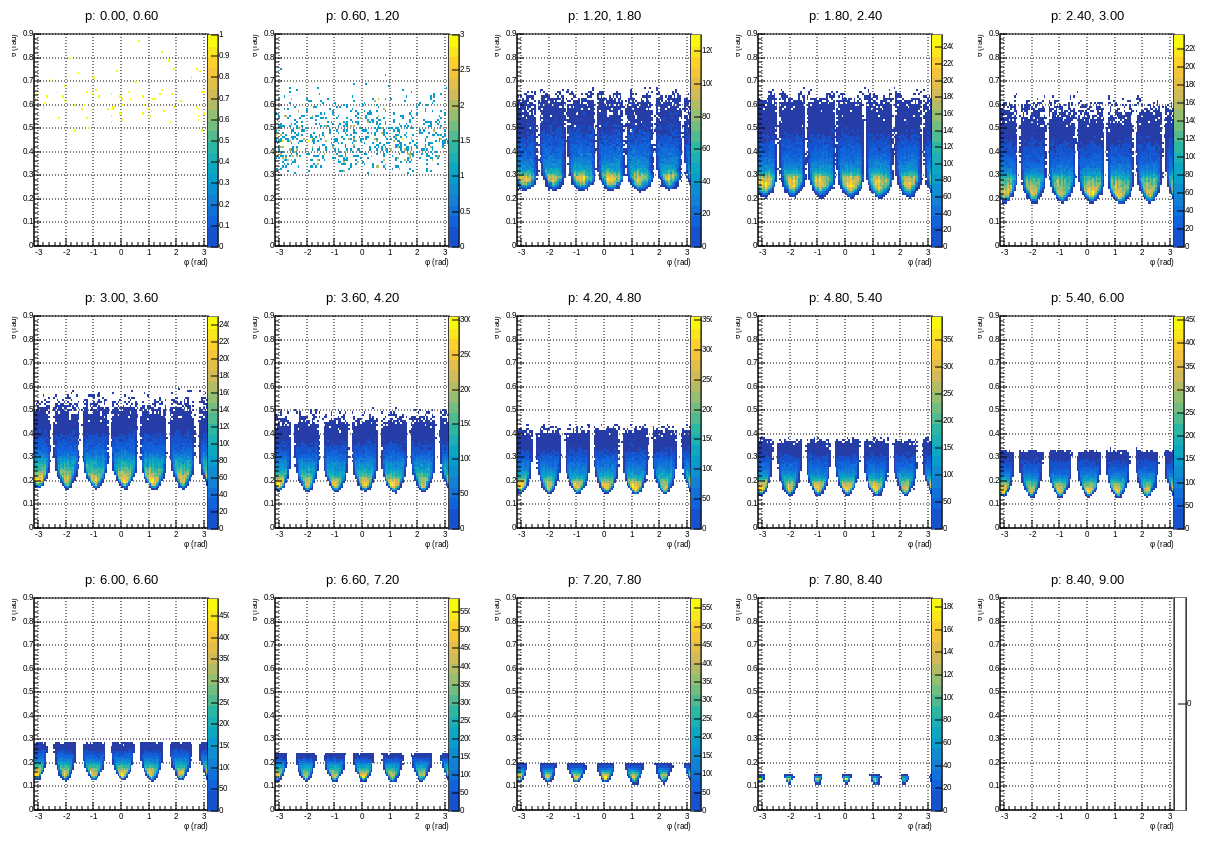
\includegraphics[width=0.70\textwidth]{06fidcuts_11.png}}
            }
        \end{figure}
        \scriptsize{\textit{
            \ef{$\phi$} vs. \ef{$\theta$} of $e^-$ detected by DC in \ef{$p$} bins. Run 12016.
        }}
    \end{center}

    \backref{11.21::summary}
\end{frame}


\subsection*{Micromegas Tracking}
% !TEX root = ../main.tex
% --+ 20.07 MICROMEGAS TRACKING +-----------------------------------------------
\begin{frame}{Micromegas Tracking}
    \label{20.07::micromegas_tracking}

    \vspace{18pt}

    \begin{columns}[onlytextwidth,T]
        \begin{column}{.34\linewidth}
            \setbeamercolor{item}{bg=color_fg,fg=color_fg}
            \begin{enumerate}
                \item[(1)]
                    \eblue{Particle} ionizes gas, creating an \ered{electron}-ion pair.

                \vspace{2pt}
                \item[(2)]
                    \egreen{$\text{E}_1$} causes the \ered{$e^-$} to drift towards the mesh.

                \vspace{2pt}
                \item[(3)]
                    \ered{$e^-$} crosses the mesh.

                \vspace{2pt}
                \item[(4)]
                    By crossing \egreen{$\text{E}_2$}, \ered{$e^-$} causes an \ered{avalanche}.

                \vspace{2pt}
                \item[(5)]
                    A significant signal is produced at the readout strip.
            \end{enumerate}
            \setbeamercolor{item}{bg=color_ef,fg=color_ef}
        \end{column}

        \begin{column}{.64\linewidth}
            \vspace{0pt}
            \begin{center}
                \fbox{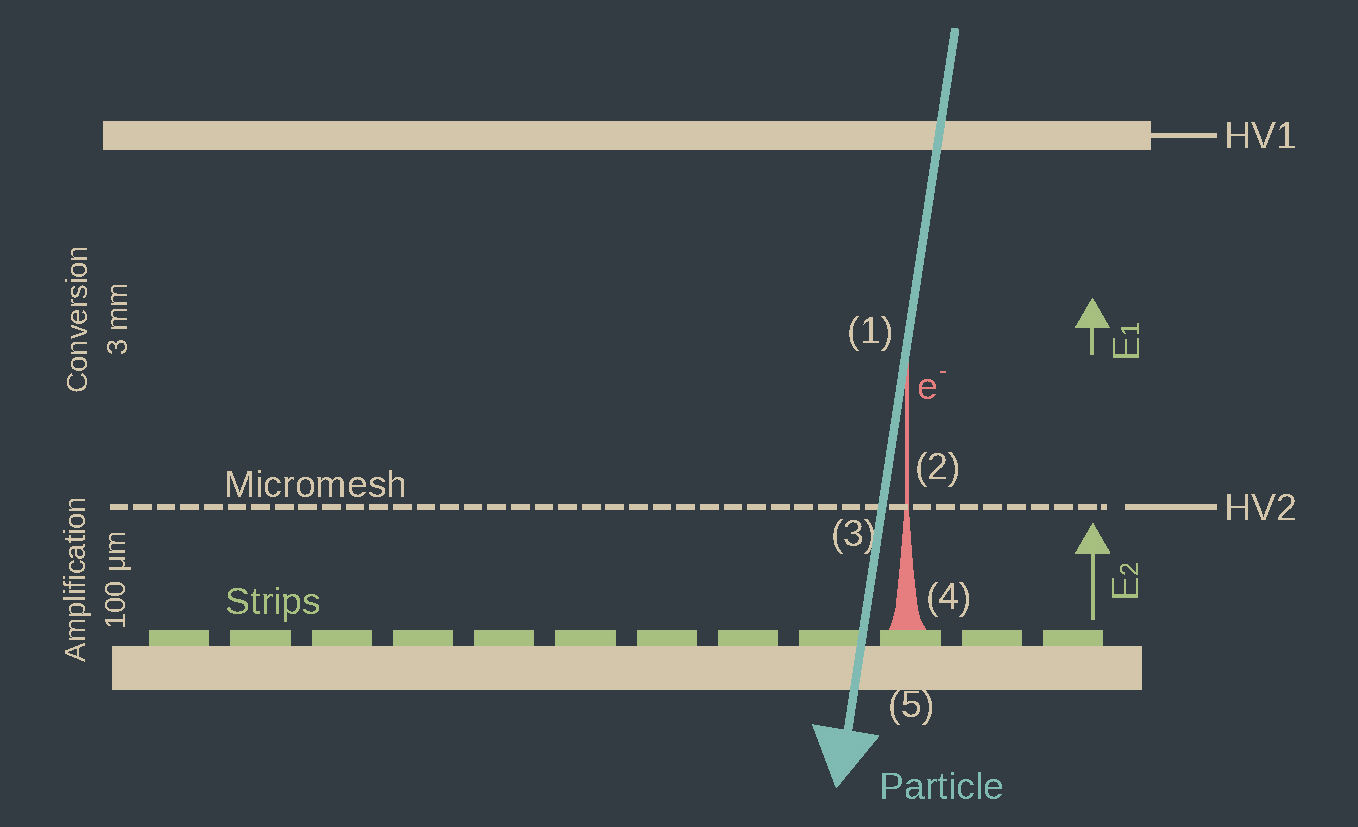
\includegraphics[width=\linewidth]{07mm_principle.pdf}}
            \end{center}
        \end{column}
    \end{columns}

    \backref{10.34::fmt}
\end{frame}


\subsection*{FMT Geometry}
% !TEX root = ../main.tex
% --+ 20.08 FMT GEOMETRY +------------------------------------------------------
\begin{frame}{FMT Geometry}
    \label{20.08::fmt_geometry}

    \vspace{6pt}

    \begin{itemize}
        \item
            To get an accurate picture of the passing particle, FMT has \ef{3 layers}.

        \item
            The $2^\text{nd}$ and $3^\text{rd}$ are rotated by \ef{$60^\circ$} in \ef{$z$} with respect to the one before.
    \end{itemize}

    \vspace{6pt}

    \begin{center}
        \fbox{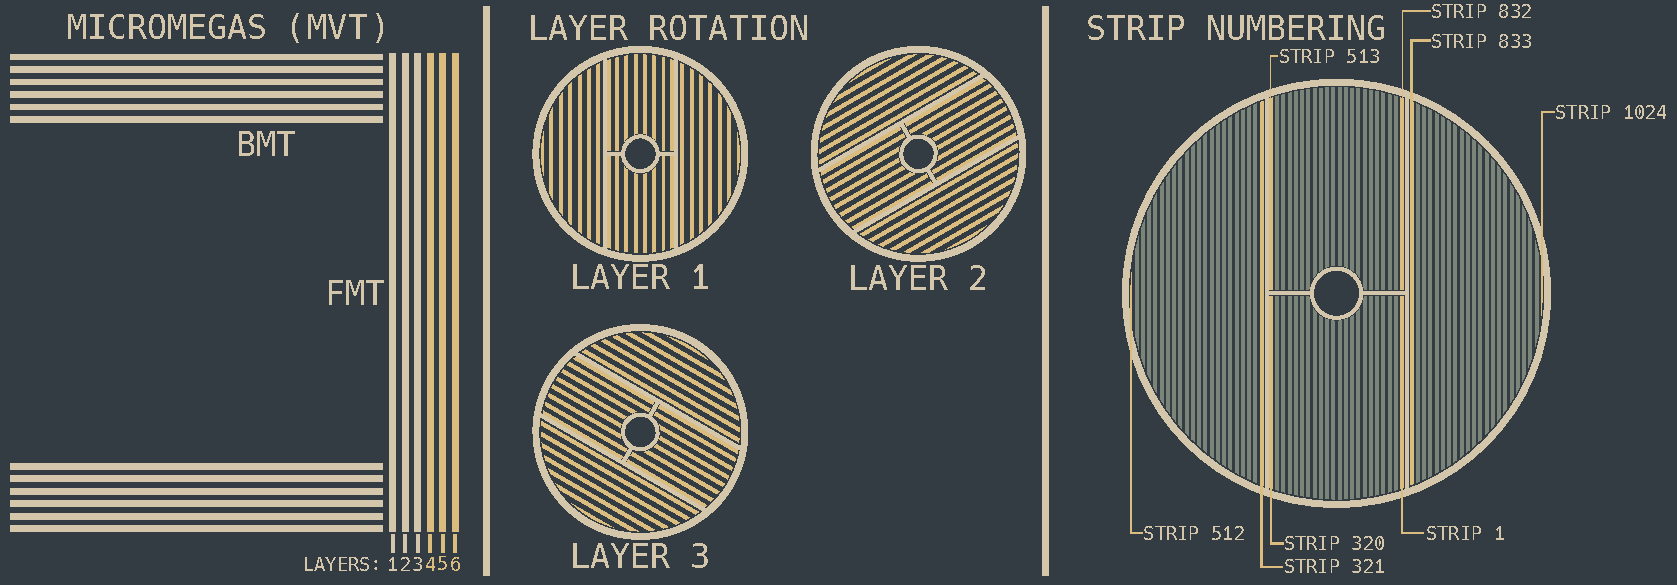
\includegraphics[width=0.98\linewidth]{08fmt_geometry.pdf}}
    \end{center}

    \backref{10.34::fmt}
\end{frame}


% --+ FMT ALIGNMENT +-----------------------------------------------------------
% --+ SYSTEMATIC ERROR ESTIMATION +---------------------------------------------
% --+ REPRODUCIBILITY +---------------------------------------------------------
% --+ UNCORRECTED DIS PLOTS +---------------------------------------------------
